%**************************************************************************************
% License:
% CC BY-NC-SA 4.0 (http://creativecommons.org/licenses/by-nc-sa/4.0/)
%**************************************************************************************

\documentclass{beamer}
\setbeameroption{hide notes}

\mode<presentation> {

\usetheme{Madrid}

% Burnt orange
\definecolor{burntorange}{rgb}{0.8, 0.33, 0.0}
\colorlet{beamer@blendedblue}{burntorange}
% Pale yellow
\definecolor{paleyellow}{rgb}{1.0, 1.0, 0.953}
\setbeamercolor{background canvas}{bg=paleyellow}
% Secondary and tertiary palette
\setbeamercolor*{palette secondary}{use=structure,fg=white,bg=burntorange!80!black}
\setbeamercolor*{palette tertiary}{use=structure,fg=white,bg=burntorange!60!black}

% Keep navigation symbols out of the content area.
\setbeamertemplate{navigation symbols}{}
}

\usepackage{amsmath}
\DeclareMathOperator*{\argmin}{arg\,min}
\DeclareMathOperator*{\argmax}{arg\,max}
\usepackage{bm}
\usepackage{booktabs} % Allows the use of \toprule, \midrule and \bottomrule in tables
\usepackage{breqn}
\usepackage{cleveref}
\usepackage{graphicx} % for figures
\usepackage[labelsep=space,tableposition=top]{caption}
\renewcommand{\figurename}{Fig.}
\usepackage{caption,subcaption}% http://ctan.org/pkg/{caption,subcaption}
\usepackage{xcolor}
\usepackage{hyperref}

\AtBeginSection[]{
	\begin{frame}[shrink=5]{Outline}
		\tableofcontents[
		currentsection,      % highlight the current section
		hideallsubsections   % show only section titles
		]
	\end{frame}
}

%----------------------------------------------------------------------------------------
%	TITLE PAGE
%----------------------------------------------------------------------------------------
\title[FNO: Operator Learning in Spectral Space]{Fourier Neural Operator: Learning Solution Operators in Spectral Space}
\author{Krishna Kumar} % name
\institute[UT Austin] % institution
{
University of Texas at Austin \\
\medskip
\textit{
  \url{krishnak@utexas.edu}} % Your email address
}
\date{} % Date, can be changed to a custom date

\begin{document}

\begin{frame}[shrink=5]
\titlepage % title page as the first slide
\end{frame}


%----------------------------------------------------------------------------------------
% slides
%----------------------------------------------------------------------------------------

\section{The Green's Function}

%------------------------------------------------
\begin{frame}
\frametitle{Learning Objectives}
\begin{itemize}
\item Write a linear solution operator as a kernel, the Green's function
\item See why translation invariance turns the kernel into a convolution
\item Follow one Fourier wave through a convolution
\item Learn the Fourier multipliers from input-output pairs
\item Stack Fourier layers and activations into an FNO
\item Train FNOs on Burgers' equation and Darcy flow
\end{itemize}
\vspace{0.3cm}
\centering
\href{https://colab.research.google.com/github/kks32-courses/sciml/blob/main/docs/05-fno/fno-intuition.ipynb}{\beamergotobutton{Heat-flow intuition}}
\href{https://colab.research.google.com/github/kks32-courses/sciml/blob/main/docs/05-fno/fno-cnn-comparisons.ipynb}{\beamergotobutton{CNN filters and Fourier multipliers}}
\href{https://colab.research.google.com/github/kks32-courses/sciml/blob/main/docs/05-fno/fno.ipynb}{\beamergotobutton{FNO}}
\end{frame}

%------------------------------------------------
\begin{frame}
\frametitle{The loaded string}
Here is a string pinned at both ends.
A load $f(x)$ pushes on it, and its displacement $u(x)$ satisfies
\[
-u''(x)=f(x),\qquad u(0)=u(1)=0.
\]
We want the whole map $f\mapsto u$, for every load at once.
\bigskip

The equation is local, because $u''$ at $x$ depends only on $u$ near $x$.
The answer is not local, because a load anywhere bends the whole string.
How does a load at one point move the rest of the string?
\end{frame}

%------------------------------------------------
\begin{frame}
\frametitle{One point load}
Put a unit load at one point $y$.
Away from $y$ there is no load, so $u''=0$ and the string is straight.
The displacement is a tent with its peak under the load,
\[
\kappa(x,y)=\begin{cases}x\,(1-y), & x\le y,\\ y\,(1-x), & x\ge y.\end{cases}
\]
\begin{center}
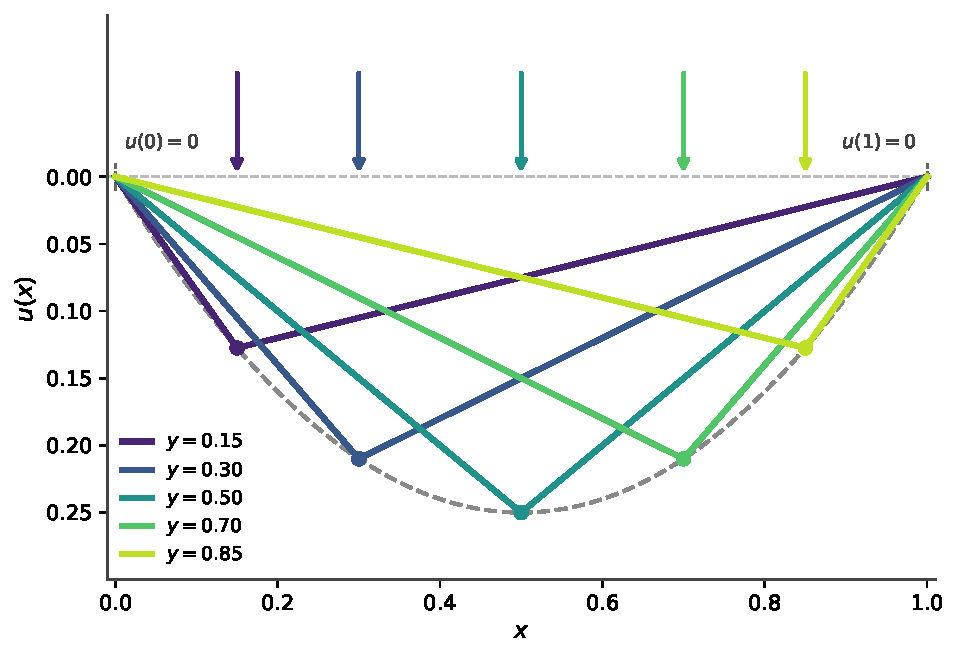
\includegraphics[width=0.62\textwidth,height=0.42\textheight,keepaspectratio]{figs/point-load-family.pdf}
\end{center}
At $y=\tfrac12$ the peak is $\tfrac14$, and the slope drops by 1 at the load.
\note{The slope is $1-y$ to the left of $y$ and $-y$ to the right, so it drops by exactly the unit load. The dashed envelope is $x(1-x)$, the peak of the tent for a load placed at $x$.}
\end{frame}

%------------------------------------------------
\begin{frame}
\frametitle{Adding up point loads}
Any load is a row of small point loads.
The piece of load near $y$ has size $f(y)\,dy$, and it makes the tent $\kappa(x,y)\,f(y)\,dy$.
Adding all the tents gives the displacement,
\[
\boxed{u(x)=\int_0^1 \kappa(x,y)\,f(y)\,dy.}
\]
Check it with a uniform load $f=1$.
The integral gives $u=\tfrac12\,x(1-x)$, and that parabola solves $-u''=1$.
\bigskip

The function $\kappa(x,y)$ is the \textbf{Green's function}.
It is the kernel of the solution operator, the response at $x$ to a unit load at $y$.
\end{frame}

%------------------------------------------------
\begin{frame}
\frametitle{The Green's matrix}
On a grid $x_1,\dots,x_N$ with spacing $h$, the integral becomes a matrix times a vector,
\[
u_i=\sum_{j=1}^N \underbrace{\kappa(x_i,y_j)\,h}_{K_{ij}}\;f_j .
\]
\begin{columns}[T]
\begin{column}{0.48\textwidth}
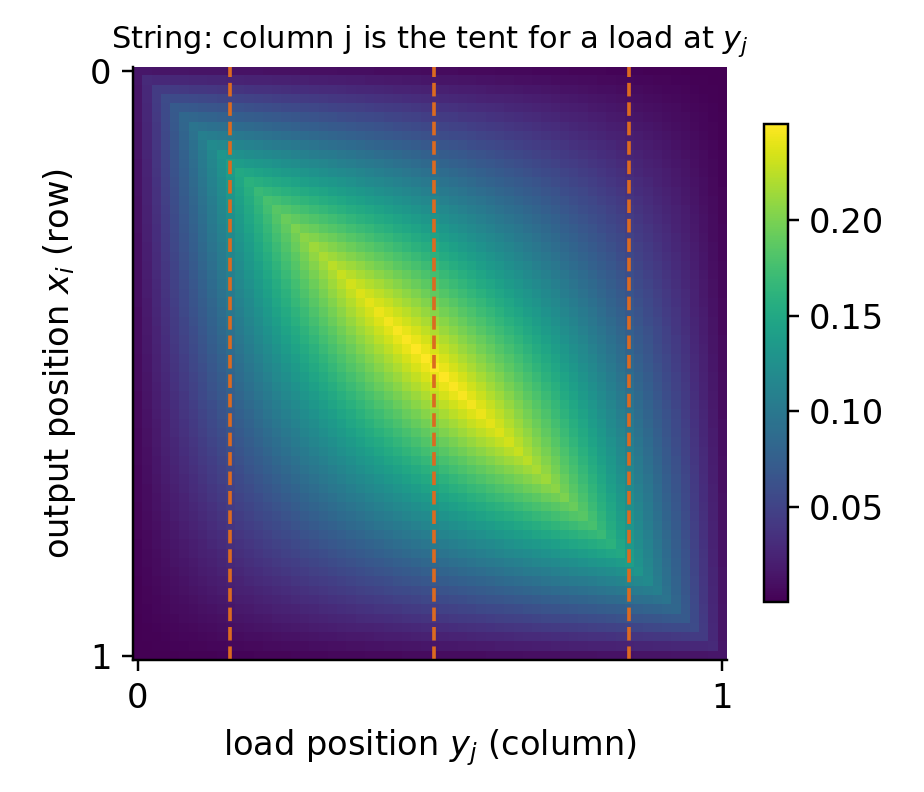
\includegraphics[width=\linewidth]{figs/string-matrix.png}
\end{column}
\begin{column}{0.5\textwidth}
\small
Column $j$ of $K$ is the tent for a load at $y_j$.
\medskip

Learning $K$ means learning $N^2$ entries.
That is 16{,}384 numbers on 128 points and about a million on 1024 points.
\medskip

Can a physical symmetry cut that number?
\end{column}
\end{columns}
\end{frame}

%------------------------------------------------
\begin{frame}
\frametitle{The shapes of the tents}
Look at the tents again.
A load near an end makes a short, lopsided tent.
A load in the middle makes the tallest tent.
\begin{center}
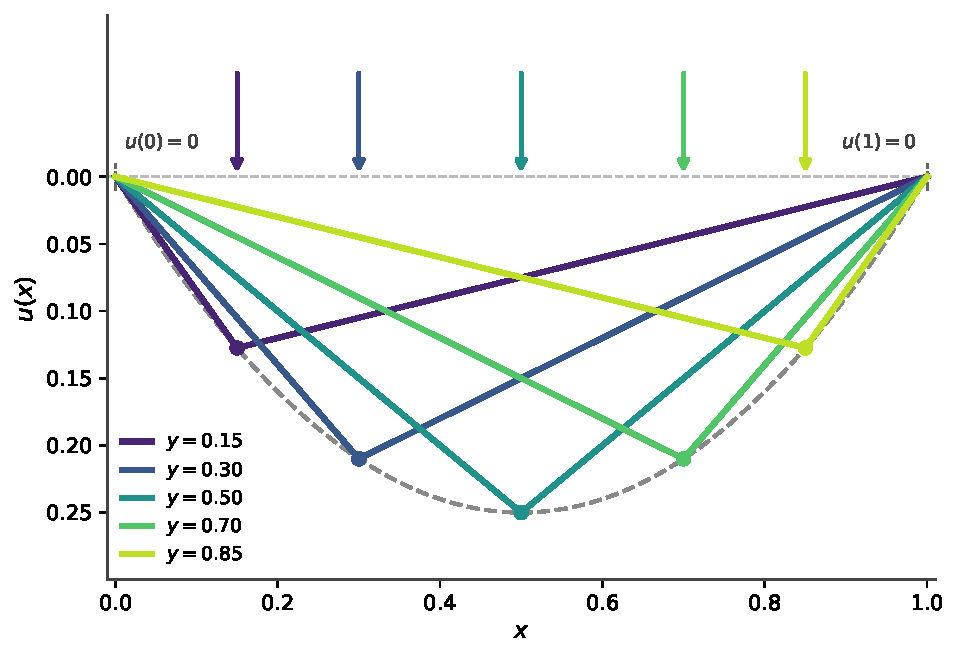
\includegraphics[width=0.5\textwidth,height=0.4\textheight,keepaspectratio]{figs/point-load-family.pdf}
\end{center}
The pinned ends make every point of the string different.
So every column of $K$ is a new shape, and we must store all of them.
What if every point of the domain looked the same?
\end{frame}

%------------------------------------------------
\section{A Ring with No Ends}

%------------------------------------------------
\begin{frame}
\frametitle{Heat on a ring}
Here is a thin metal ring with temperature $u(x)$ at the angle $x\in[0,2\pi)$.
Heat flows for a time $T$ according to $u_t=\nu u_{xx}$, with $\nu=0.14$ and $T=0.65$.
Every point of the ring looks the same, and heat flow on it has a solution we can write down.
Put one unit of heat at the point $y$ and let it flow.
\begin{center}
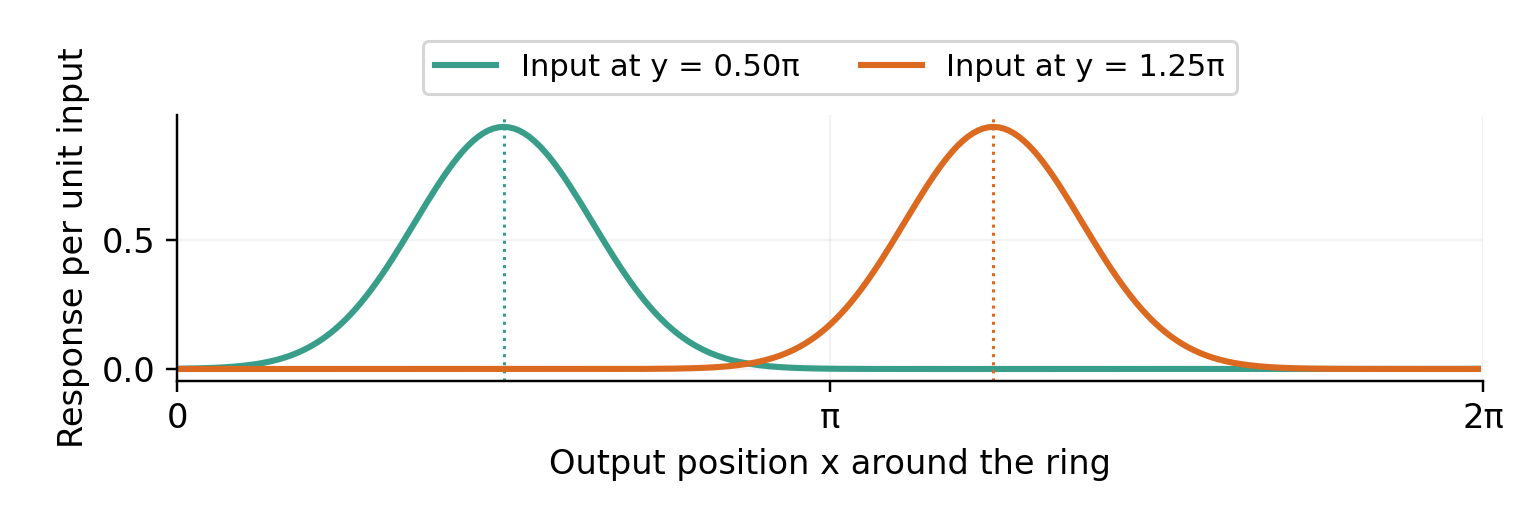
\includegraphics[width=0.92\textwidth,height=0.4\textheight,keepaspectratio]{figs/heat-point-influence.png}
\end{center}
The heat spreads into a bump centered at $y$.
Move $y$, and the bump moves with it and keeps its shape.
\end{frame}

%------------------------------------------------
\begin{frame}
\frametitle{The ring's matrix}
The ring has no ends, so the response at $x$ depends only on how far $x$ is from $y$,
\[
\kappa(x,y)=\kappa(x-y),
\]
with the separation $x-y$ measured around the ring.
\begin{columns}[T]
\begin{column}{0.48\textwidth}
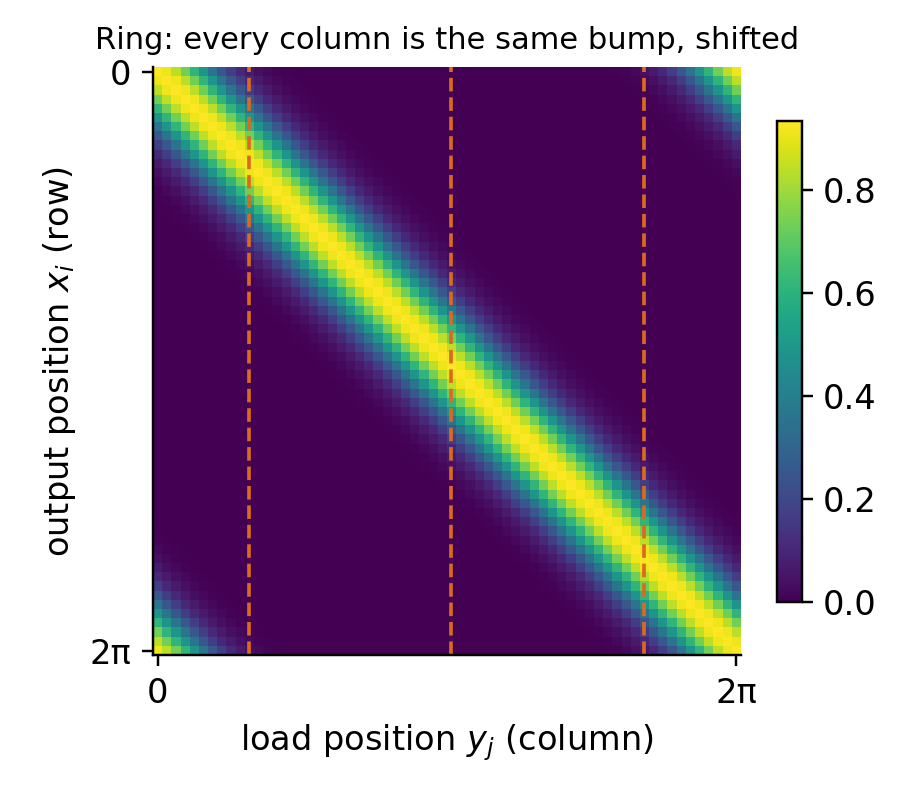
\includegraphics[width=\linewidth]{figs/ring-matrix.png}
\end{column}
\begin{column}{0.5\textwidth}
\small
Every column of the ring's matrix is the same bump, shifted down by one grid point.
The bump wraps around at the bottom.
\medskip

One column of $N$ numbers now determines all $N^2$ entries.
A matrix with this structure is \textbf{circulant}.
\end{column}
\end{columns}
\end{frame}

%------------------------------------------------
\begin{frame}
\frametitle{A convolution}
Adding up point sources on the ring now gives
\[
\boxed{u(x,T)=\int_0^{2\pi} \kappa(x-y)\,u_0(y)\,dy.}
\]
This integral is the \textbf{convolution} of the initial temperature $u_0$ with the kernel $\kappa$.
It slides one fixed shape $\kappa$ around the ring and weights it by $u_0$.
\bigskip

A general Green's function depends on $x$ and $y$ separately.
Boundaries, as on the string, and a conductivity that changes with $x$ both prevent the convolution form.
The Fourier layer is built for the convolution case.
\end{frame}

%------------------------------------------------
\begin{frame}
\frametitle{A CNN filter on the ring}
A CNN computes the same kind of sum with a short filter.
The blur on a ring of six points is a circulant matrix,
\[
\begin{bmatrix}y_1\\y_2\\y_3\\y_4\\y_5\\y_6\end{bmatrix}
=\frac13
\begin{bmatrix}
1&1&0&0&0&1\\
1&1&1&0&0&0\\
0&1&1&1&0&0\\
0&0&1&1&1&0\\
0&0&0&1&1&1\\
1&0&0&0&1&1
\end{bmatrix}
\begin{bmatrix}u_1\\u_2\\u_3\\u_4\\u_5\\u_6\end{bmatrix}.
\]
Each row is the row above, shifted one place.
Shifting the input shifts the output, as on the ring.
\note{This is translation equivariance for stride 1 and periodic padding. Pooling and classification invariance are separate questions. Stacked local layers can produce a larger receptive field.}
\end{frame}

%------------------------------------------------
\begin{frame}
\frametitle{The width of the heat kernel}
The heat kernel is a Gaussian with standard deviation $\sqrt{2\nu T}=0.43$.
On 128 points the spacing is $2\pi/128=0.049$, so the kernel is 8.7 spacings wide.
\begin{center}
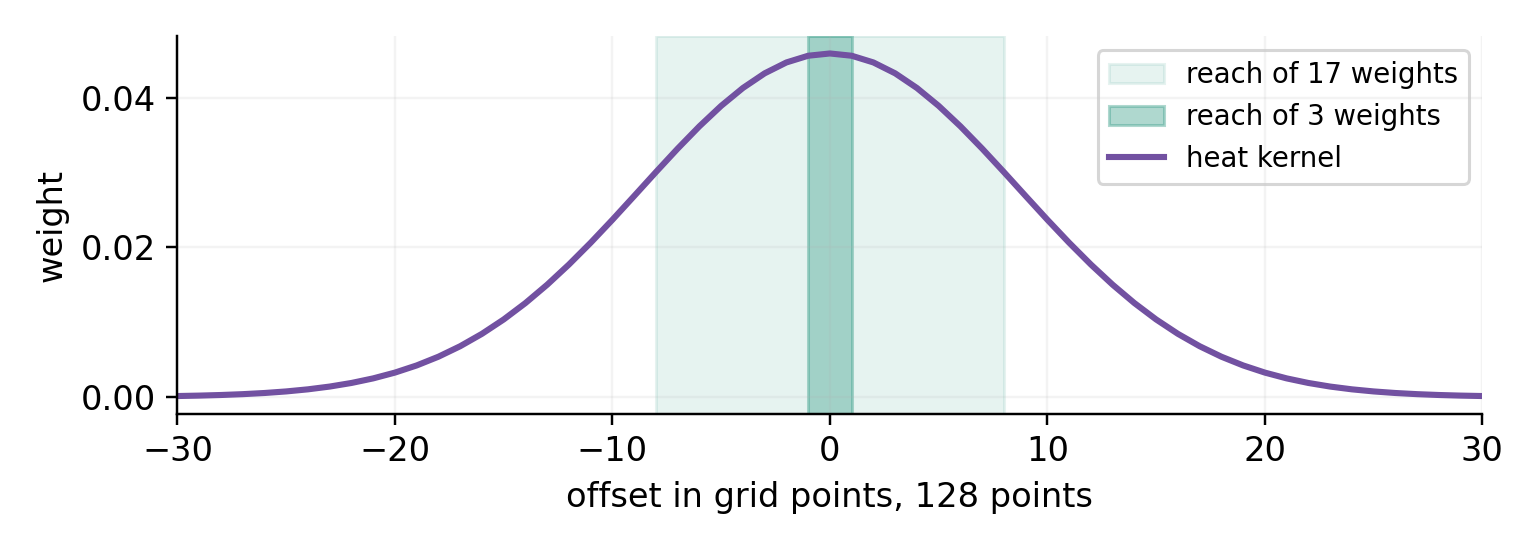
\includegraphics[width=0.8\textwidth,height=0.3\textheight,keepaspectratio]{figs/cnn-reach.png}
\end{center}
\small
\begin{center}
\begin{tabular}{lcccc}
\toprule
CNN weights, fitted to 64 heat pairs & 3 & 9 & 17 & 25\\
Held-out relative error & 0.63 & 0.098 & 0.0035 & 0.00066\\
\bottomrule
\end{tabular}
\end{center}
A wider filter works, but on 256 points the same kernel is 17.4 spacings wide.
Can we describe the kernel with numbers that do not count grid points?
\end{frame}

%------------------------------------------------
\section{Waves Through a Convolution}

%------------------------------------------------
\begin{frame}
\frametitle{One wave through three filters}
Try the simplest input, the single wave $\sin 7x$ on 32 points.
Apply three image filters, the blur, the shift, and the sharpening filter.
\begin{center}
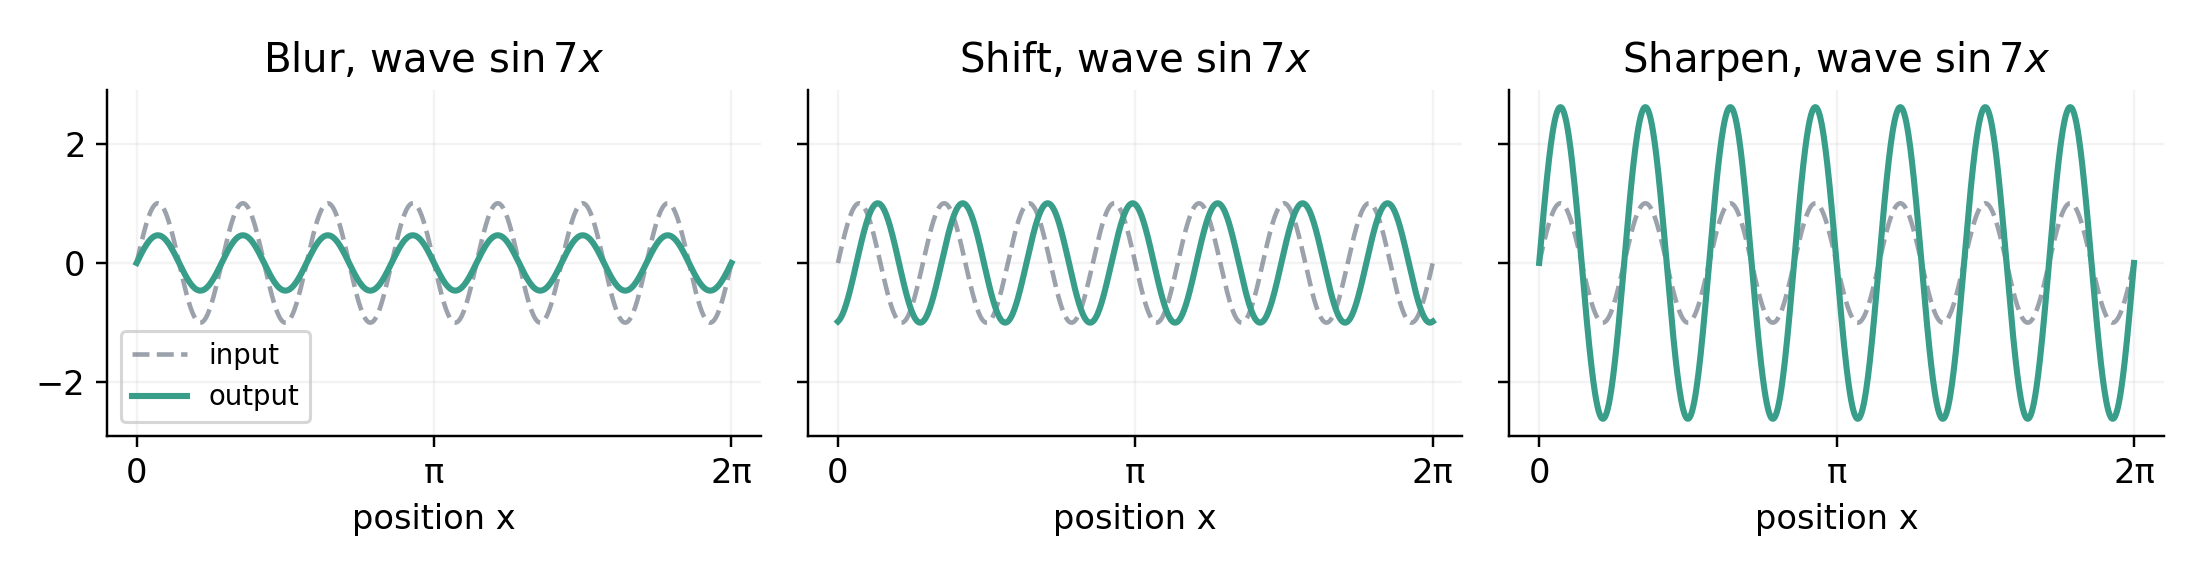
\includegraphics[width=\textwidth,height=0.36\textheight,keepaspectratio]{figs/filters-on-a-wave.png}
\end{center}
The blur makes the wave smaller.
The sharpening filter makes it larger.
The shift moves it sideways.
Every output is still a wave with seven periods, so no filter changed the frequency.
\end{frame}

%------------------------------------------------
\begin{frame}
\frametitle{The multiplier of a wave}
Write the wave as $e^{ikx}$.
Moving it by $s$ multiplies it by one number,
\[
e^{ik(x-s)}=e^{-iks}\,e^{ikx}.
\]
A convolution adds moved copies, so it also multiplies the wave by one number,
\[
\int \kappa(s)\,e^{ik(x-s)}\,ds=\underbrace{\Big(\int \kappa(s)\,e^{-iks}\,ds\Big)}_{R(k)}\,e^{ikx}.
\]
The number $R(k)$ is the \textbf{multiplier} of mode $k$.
\medskip

Check it on the blur, which adds three copies moved by $-1$, $0$, and $1$ grid points.
Its multiplier is $R(k)=\tfrac13(1+2\cos\theta_k)$ with $\theta_k=2\pi k/N$.
For $\sin7x$ on 32 points, $\theta_7=1.37$ and $\cos\theta_7=0.20$, so the blur multiplies the wave by 0.46.
\end{frame}

%------------------------------------------------
\begin{frame}
\frametitle{The multipliers of three filters}
\begin{center}
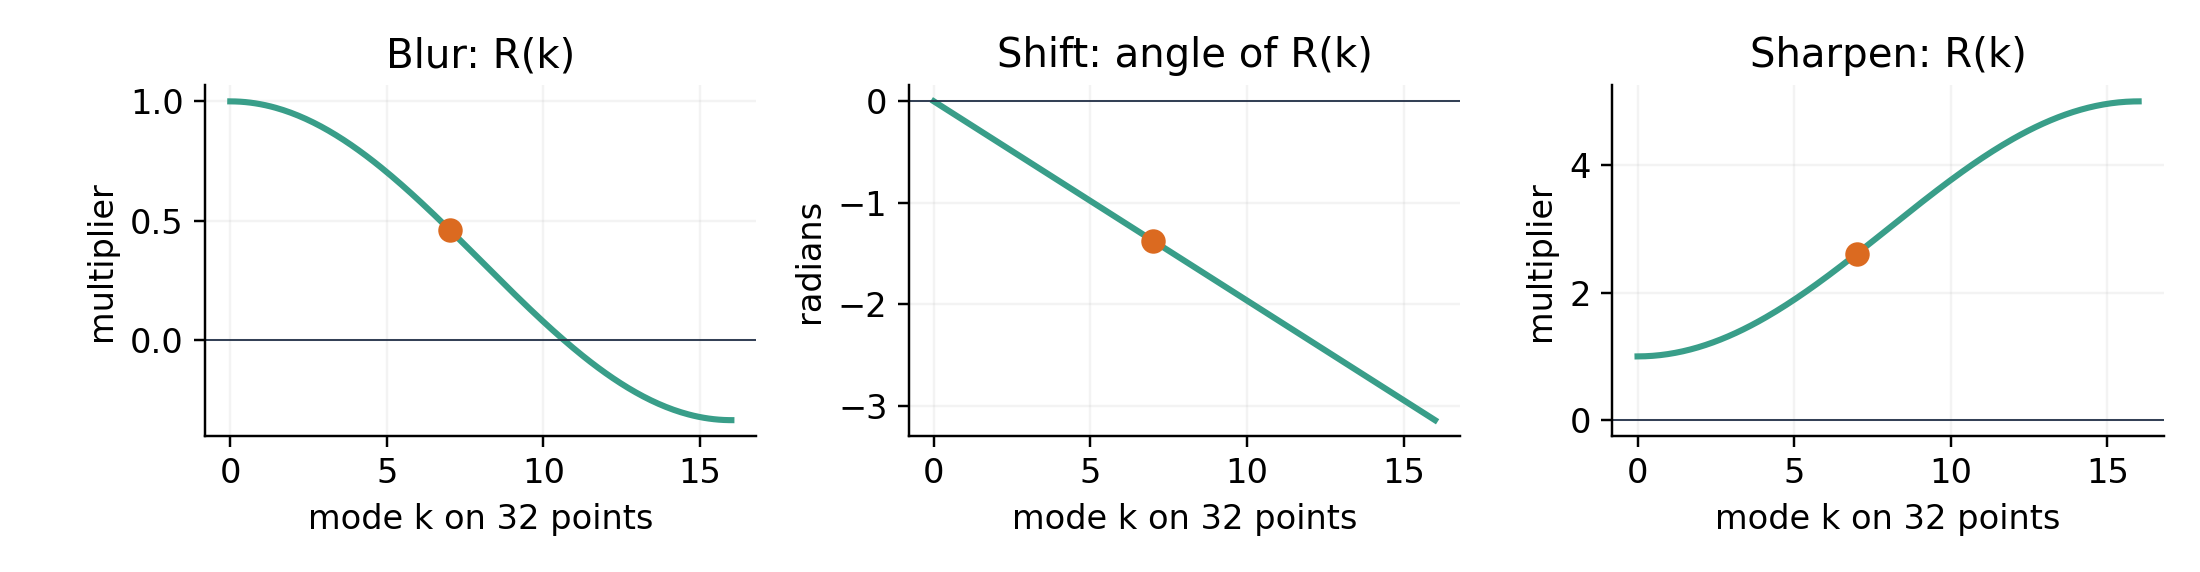
\includegraphics[width=\textwidth,height=0.38\textheight,keepaspectratio]{figs/filter-responses.png}
\end{center}
The orange dots are the wave $\sin7x$ from the last slide.
\begin{itemize}
\item The blur's multiplier falls with $k$, so it shrinks fast waves.
\item The sharpening multiplier rises toward 5, so it strengthens fast waves.
\item The shift keeps every size at 1 and turns the phase by $\theta_k$.
\end{itemize}
All three multipliers equal 1 at $k=0$, so all three filters leave a constant unchanged.
\end{frame}

%------------------------------------------------
\begin{frame}
\frametitle{The multipliers of heat flow}
Heat flow on the ring is a convolution, so it also multiplies each wave by one number.
Put $u=q_k(t)\,e^{ikx}$ into $u_t=\nu u_{xx}$,
\[
\frac{dq_k}{dt}=-\nu k^2q_k,\qquad R(k)=e^{-\nu k^2T}.
\]
\begin{center}
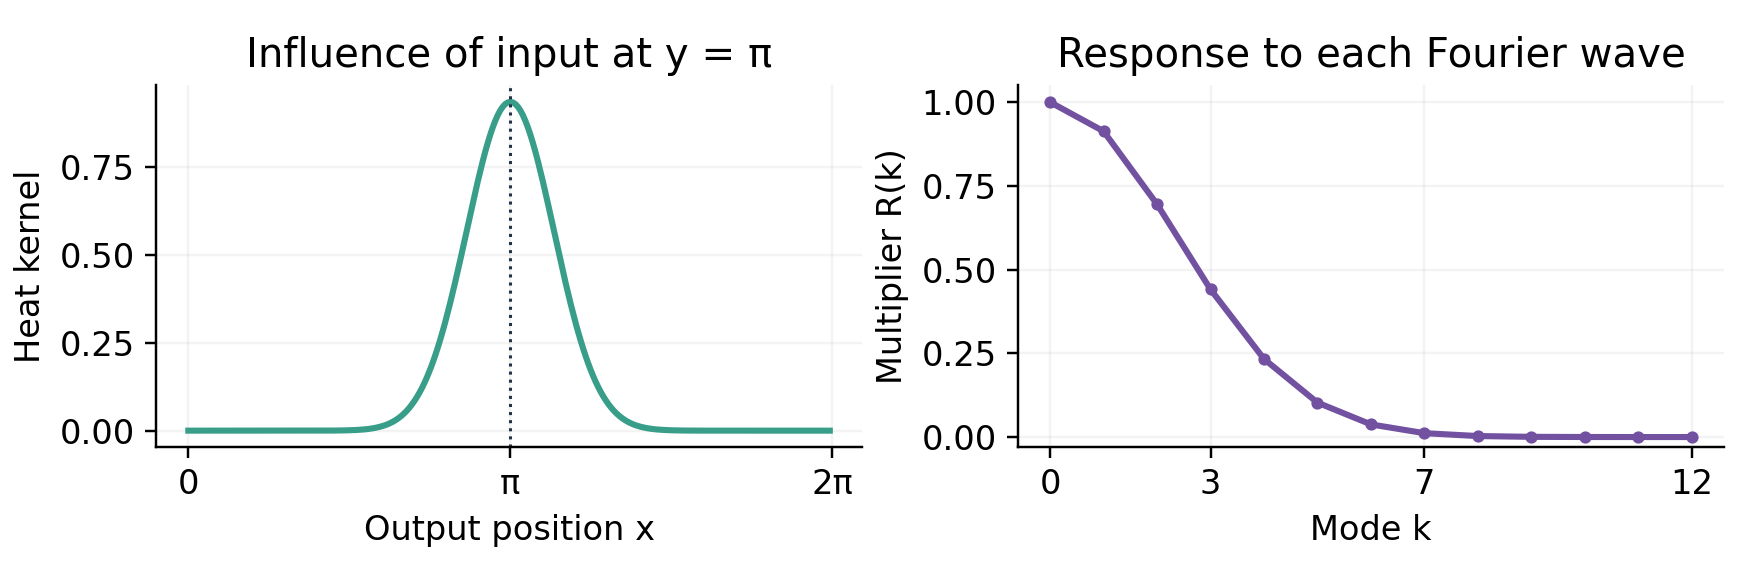
\includegraphics[width=0.9\textwidth,height=0.36\textheight,keepaspectratio]{figs/heat-kernel-multiplier.png}
\end{center}
With $\nu T=0.091$, the multiplier is 0.913 at $k=1$, 0.441 at $k=3$, and 0.0116 at $k=7$.
Fast waves have more curvature, so they decay first.
\end{frame}

%------------------------------------------------
\begin{frame}
\frametitle{Fourier coordinates on the ring}
A field on the ring is a sum of waves with amplitudes $\widehat v_k$,
\[
v(x)=\sum_{k\in\mathbb Z}\widehat v_k\,e^{ikx},
\qquad
\widehat v_k=\frac{1}{2\pi}\int_0^{2\pi}v(x)\,e^{-ikx}\,dx.
\]
On the grid $x_j=2\pi j/N$, the FFT computes the amplitudes from the heights,
\[
\widehat v_k=\frac1N\sum_{j=0}^{N-1}v(x_j)\,e^{-ikx_j}.
\]
The heights $v(x_j)$ and the amplitudes $\widehat v_k$ are two lists that describe the same field.
The FFT and its inverse convert one list into the other in $O(N\log N)$ operations.
\note{The finite-grid formula gives the coefficients of the trigonometric interpolant. Resolving the input and the products formed by nonlinear terms is a separate discretization question.}
\end{frame}

%------------------------------------------------
\begin{frame}
\frametitle{Three waves}
\begin{center}
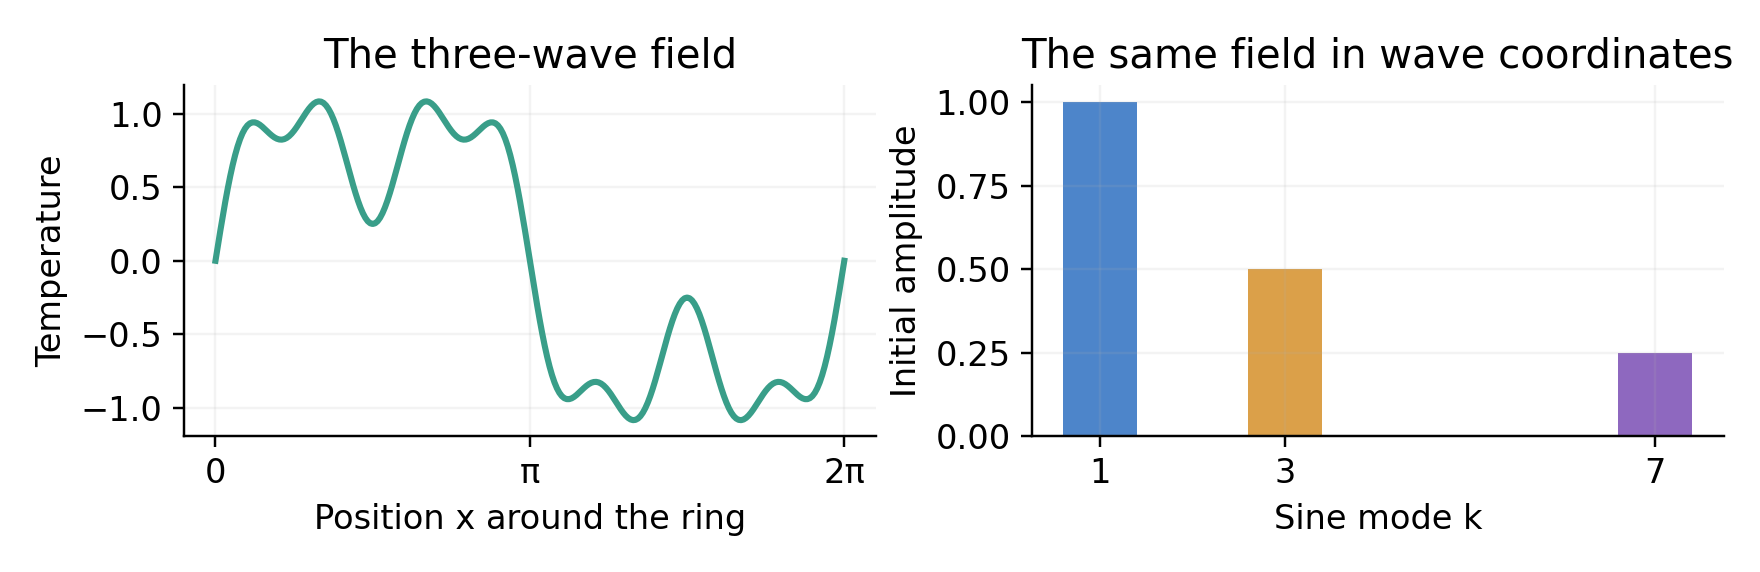
\includegraphics[width=\textwidth,height=0.40\textheight,keepaspectratio]{figs/fno-three-wave-coordinates.png}
\end{center}
Take $u_0=\sin x+\tfrac12\sin3x+\tfrac14\sin7x$.
Heat flow multiplies each amplitude by its own number,
\[
\begin{bmatrix}q_1(T)\\q_3(T)\\q_7(T)\end{bmatrix}
=\operatorname{diag}(0.913,\,0.441,\,0.0116)
\begin{bmatrix}1\\0.5\\0.25\end{bmatrix}.
\]
The amplitude of mode 3 goes from 0.5 to $0.5\times0.441\approx0.220$.
\end{frame}

%------------------------------------------------
\begin{frame}
\frametitle{One operator in two bases}
The heights and the wave amplitudes are two coordinate systems for the same field.
Choosing the Fourier waves is a change of basis, as choosing any other basis is.
The basis alone does not make the Fourier layer.
What matters is the matrix of the operator in that basis.
\begin{center}
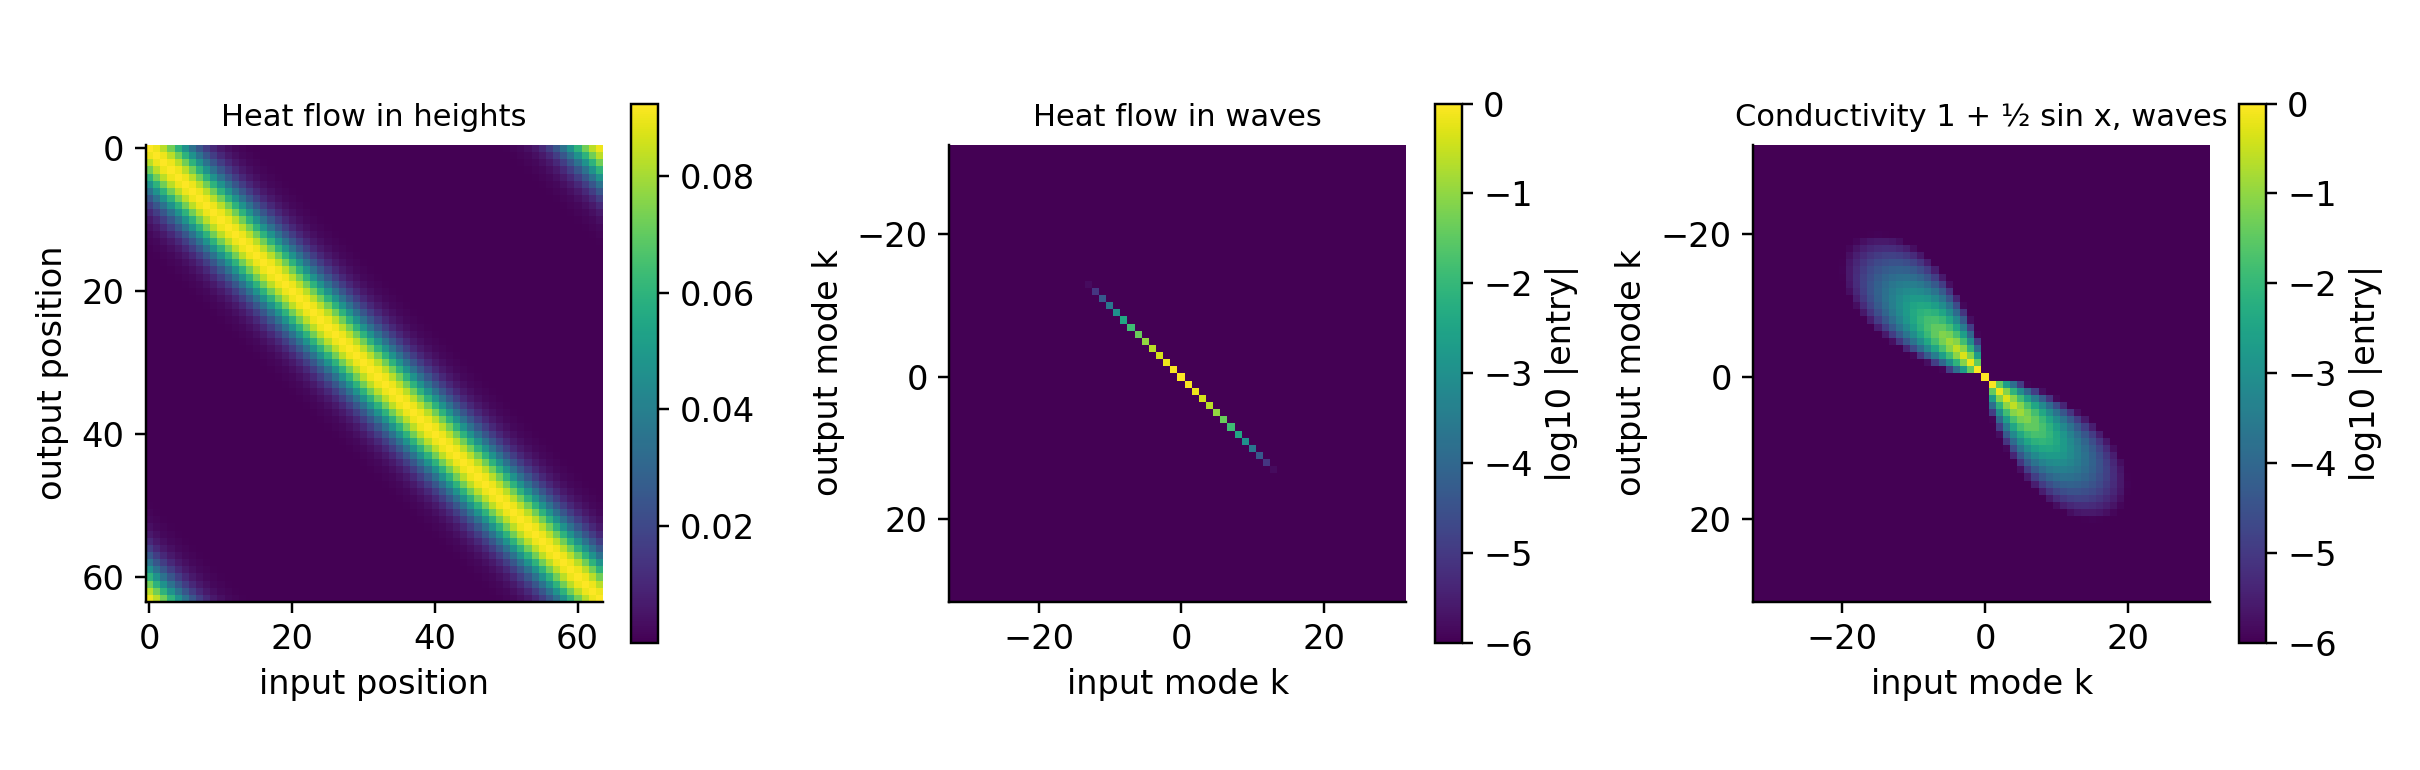
\includegraphics[width=\textwidth,height=0.38\textheight,keepaspectratio]{figs/operator-in-two-bases.png}
\end{center}
\small
In heights, heat flow is a dense circulant matrix.
In waves, the same operator is diagonal, so output mode $k$ uses input mode $k$ alone.
A conductivity $1+\tfrac12\sin x$ breaks the shift symmetry, and the matrix in waves is no longer diagonal.
\note{All three matrices use 64 points and the same finite-volume diffusion, with nu T = 0.091. The largest off-diagonal entry in waves is 8.8e-16 for constant conductivity and 0.09 for the conductivity 1 + sin(x)/2. The colors in the two right panels are log10 of the magnitude.}
\end{frame}

%------------------------------------------------
\begin{frame}
\frametitle{Convolution by FFT}
A field is a sum of waves, and a convolution acts on each wave by itself.
So three steps compute the convolution,
\[
\boxed{u(\cdot,T)=\mathcal F^{-1}\big[R(k)\,\mathcal F(u_0)\big].}
\]
\begin{enumerate}
\item The FFT finds the amplitude of each wave in $u_0$.
\item Multiply amplitude $k$ by $R(k)$.
\item The inverse FFT adds the changed waves back together.
\end{enumerate}
\bigskip
The kernel matrix has $N^2$ entries.
The multipliers are $N/2+1$ numbers, and they refer to modes, not to grid points.
\end{frame}

%------------------------------------------------
\section{Learning the Multipliers}

%------------------------------------------------
\begin{frame}
\frametitle{Multipliers from data}
Now suppose we do not know $\nu$.
We have 64 pairs of initial and final profiles on 128 points, made of modes 0 to 12.
For every pair $j$, mode $k$ obeys $b_k^{(j)}=R(k)\,a_k^{(j)}$, so the pairs lie on a line through the origin.
\begin{center}
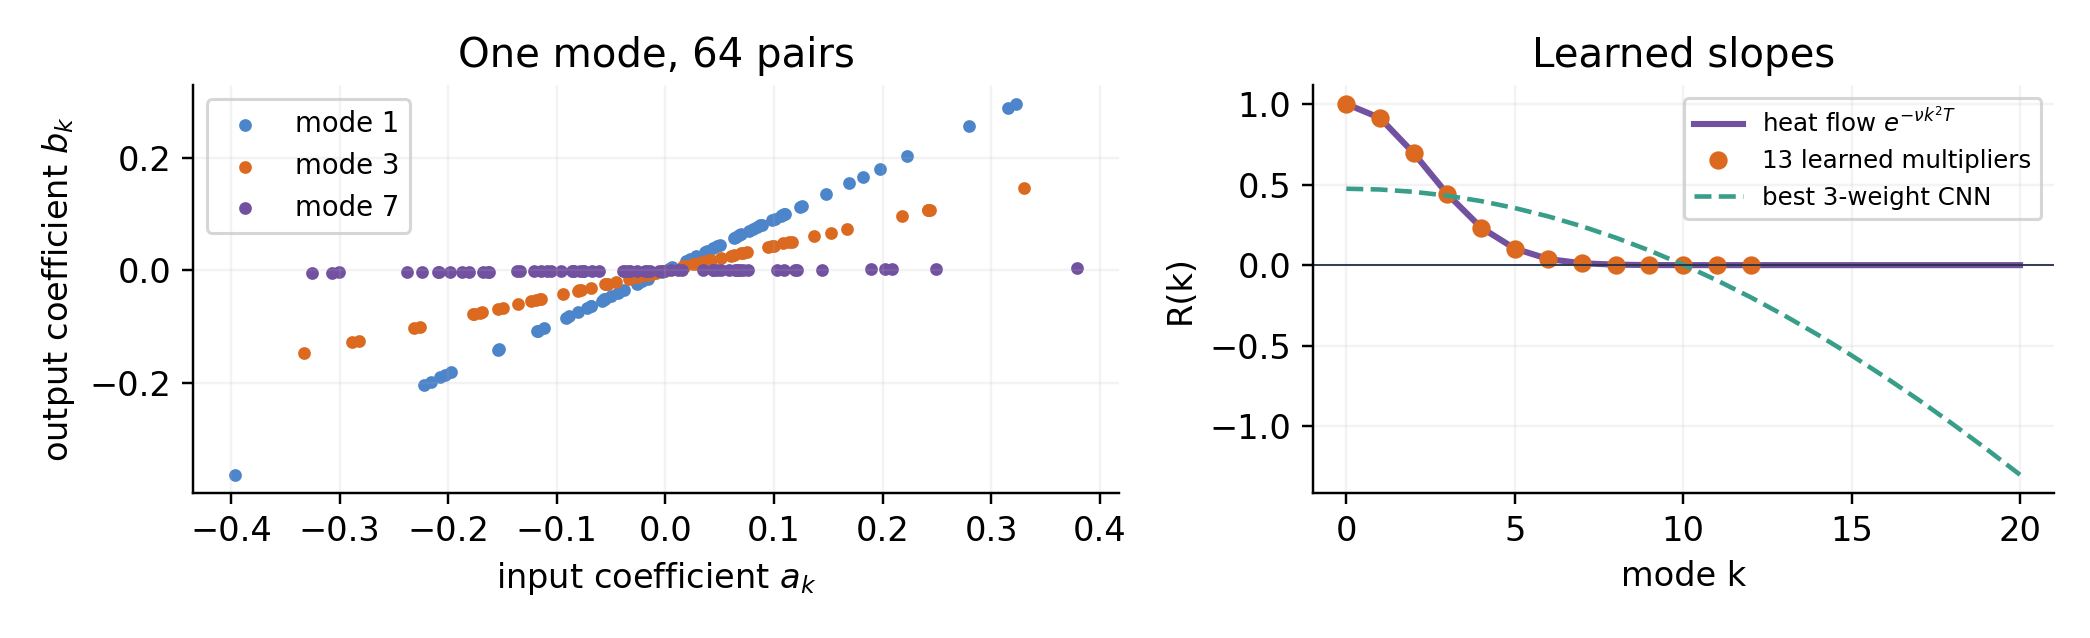
\includegraphics[width=\textwidth,height=0.38\textheight,keepaspectratio]{figs/learned-multipliers.png}
\end{center}
Least squares fits the slope of each mode,
$R(k)=\sum_j \overline{a_k^{(j)}}\,b_k^{(j)}\big/\sum_j |a_k^{(j)}|^2$.
The 13 fitted numbers match $e^{-\nu k^2T}$, and the held-out error is $2.2\times10^{-16}$.
The best three-weight CNN is the dashed cosine, which cannot follow the heat curve.
\end{frame}

%------------------------------------------------
\begin{frame}
\frametitle{The kernel of a Fourier layer}
A Fourier layer keeps a set $\mathcal M$ of low modes and sets the others to zero,
\[
\mathcal K v=\mathcal F^{-1}\big[R(k)\,\widehat v_k\big],\qquad k\in\mathcal M.
\]
In space, the layer is a convolution with the kernel
\[
\kappa(s)=\frac1{2\pi}\sum_{k\in\mathcal M}R(k)\,e^{iks},
\]
and every retained wave extends around the whole ring.
\begin{center}
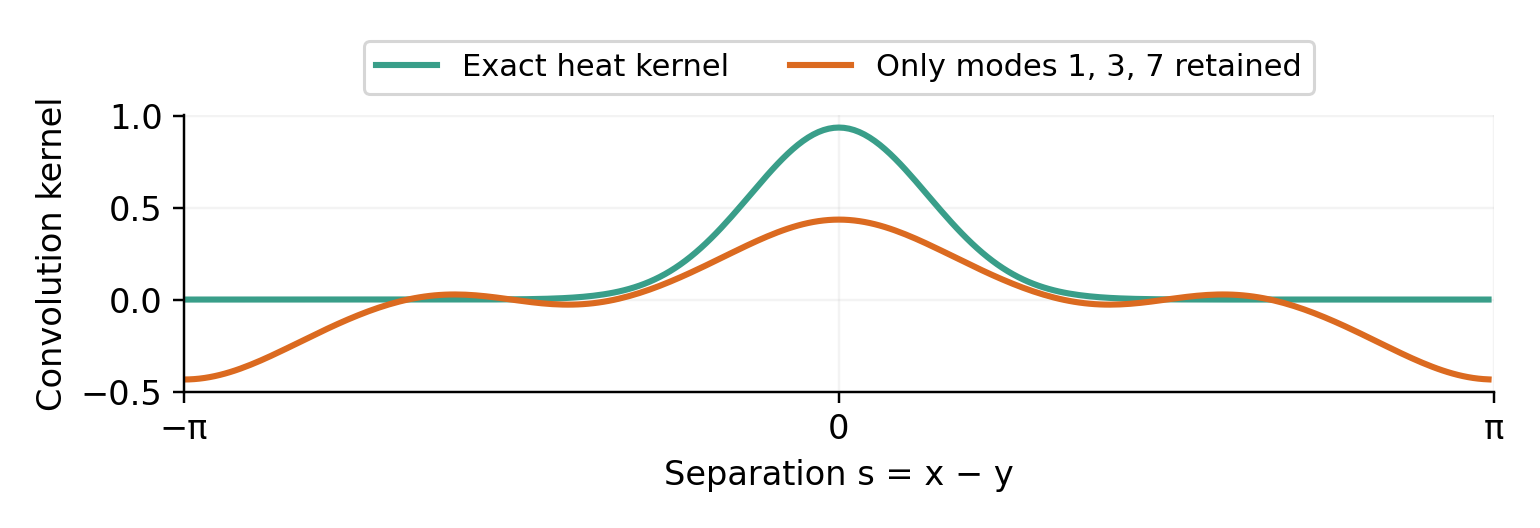
\includegraphics[width=0.78\textwidth,height=0.3\textheight,keepaspectratio]{figs/heat-retained-kernel.png}
\end{center}
\small
With only modes 1, 3, and 7 kept, the kernel differs from the heat kernel.
It gives the same output for every field made of those three modes.
\smallskip

\footnotesize\href{https://arxiv.org/abs/2010.08895}{Li et al., Fourier Neural Operator, Section 4.}
\note{The kernel formula uses normalized Fourier-series coefficients for fields and an unnormalized integral for the convolution multiplier. A real kernel requires R(-k)=conj(R(k)). For channel-valued features the kernel and multipliers are matrices.}
\end{frame}

%------------------------------------------------
\begin{frame}
\frametitle{Finer grids}
A CNN's multiplier depends on the grid through $\theta_k=2\pi k/N$.
On 256 points, mode $k$ sits where mode $k/2$ sat on 128 points.
So a CNN trained on 128 points applies $e^{-\nu(k/2)^2T}=e^{-\nu k^2(T/4)}$, which is heat flow for the time $T/4$.
The learned multiplier $R(k)$ is indexed by $k$ itself.
\medskip
\begin{center}
\small
\begin{tabular}{cccc}
\toprule
Points & Fourier layer vs $T$ & 17-weight CNN vs $T$ & 17-weight CNN vs $T/s$\\
\midrule
128 & $2.2\times10^{-16}$ & 0.0035 & 0.0035, $s=1$\\
256 & $2.1\times10^{-16}$ & 0.78 & 0.0028, $s=4$\\
512 & $2.2\times10^{-16}$ & 1.7 & 0.0021, $s=16$\\
\bottomrule
\end{tabular}
\end{center}
\medskip
Both maps were trained once on 128 points.
The transfer works because the test profiles contain only modes 0 to 12 and every grid resolves them.
\end{frame}

%------------------------------------------------
\section{From One Layer to the FNO}

%------------------------------------------------
\begin{frame}
\frametitle{Squaring a wave}
Every map so far multiplies waves that are already in the input.
Now square $\sin x$,
\[
\sin^2x=\tfrac12-\tfrac12\cos2x.
\]
\begin{center}
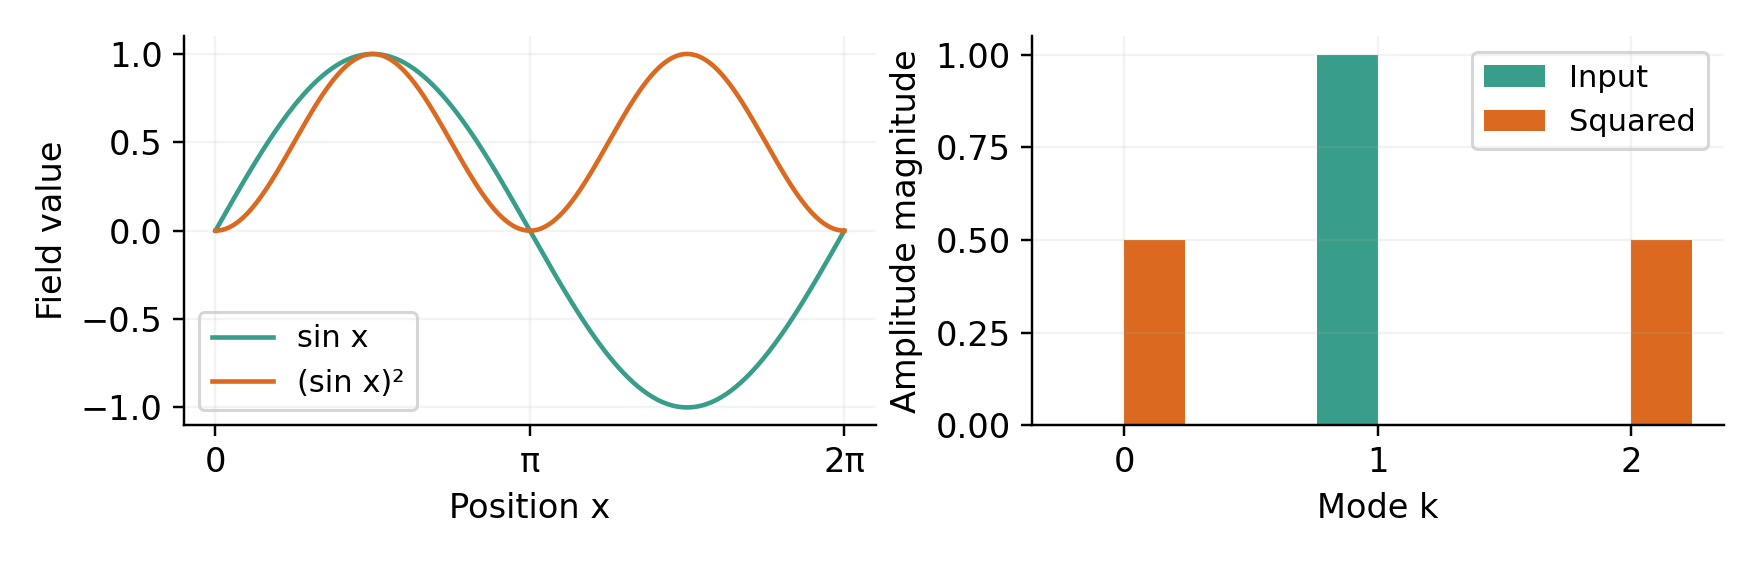
\includegraphics[width=0.98\textwidth,height=0.4\textheight,keepaspectratio]{figs/fourier-new-modes.png}
\end{center}
The square contains modes 0 and 2, and the input contained only mode 1.
A multiplier gives $R(2)\times0=0$, so no multiplier can create mode 2.
A pointwise nonlinear operation can.
\note{The bars show real sine and cosine amplitude magnitudes. The constant is mode zero. A generic activation need not equal squaring, but it can introduce new frequencies.}
\end{frame}

%------------------------------------------------
\begin{frame}
\frametitle{One FNO block}
An FNO block sends a feature field $v_\ell(x)$ down two paths and adds them,
\begin{align*}
z(x)&=\mathcal F^{-1}[R_\ell\,\mathcal F(v_\ell)](x) && \text{global, the learned multipliers}\\
y(x)&=W_\ell\,v_\ell(x)+b_\ell && \text{local, at each point}\\
v_{\ell+1}(x)&=\sigma\bigl(z(x)+y(x)\bigr) && \text{pointwise activation}
\end{align*}
\begin{itemize}
\item The spectral path multiplies mode $k$ by $R_\ell(k)$, which couples every point of the domain.
\item The local path multiplies every mode by the same matrix $W_\ell$, and it keeps modes that the spectral cutoff drops.
\item Both linear paths act on each mode separately. Only the activation $\sigma$ couples different modes.
\end{itemize}
In two dimensions, $k$ is a vector and the same formulas apply.
\end{frame}

%------------------------------------------------
\begin{frame}
\frametitle{Channels}
A feature field has $C$ channels at each point, so $R_\ell(k)$ is a $C\times C$ matrix,
\[
\widehat z_o(k)=\sum_{i=1}^{C}R_{oi}(k)\,\widehat v_i(k),
\qquad k\in\mathcal M.
\]
At a fixed mode $k$, the matrix mixes the channels.
Different modes still do not mix.
\bigskip

Count the numbers in one 1D layer of the Burgers model, with $C=64$ channels and 16 retained modes.
The spectral path has $64\times64\times16=65{,}536$ complex multipliers.
That count does not change when the grid is refined.
\end{frame}


%------------------------------------------------
\begin{frame}
\frametitle{Complete FNO Architecture}
\begin{figure}[ht]
    \centering
    \includegraphics[width=0.9\textwidth]{figs/fourier_architecture.png}
    \caption*{Fourier Neural Operator architecture.}
\end{figure}
\begin{itemize}
    \item The lifting $P$ maps the input at each point to $C$ channels, $v_0=P(u)$.
    \item Four Fourier blocks compute $v_{\ell+1}=\sigma(W_\ell v_\ell+b_\ell+\mathcal K_\ell v_\ell)$.
    \item The projection $Q$ maps the $C$ channels at each point to the output.
\end{itemize}
\end{frame}

%------------------------------------------------
\begin{frame}
\frametitle{Pseudospectral evaluation and an FNO block}
\small
\begin{columns}[T]
\begin{column}{0.48\textwidth}
\textbf{Pseudospectral Burgers}
\begin{enumerate}
\item Start with coefficients of $u$.
\item Apply known multipliers $1$ and $ik$.
\item IFFT to values of $u$ and $u_x$.
\item Form the product $u\,u_x$ on the grid.
\item FFT the product and integrate the PDE in time.
\end{enumerate}
\end{column}
\begin{column}{0.48\textwidth}
\textbf{FNO features}
\begin{enumerate}
\item Start with a feature field $v_\ell$.
\item FFT and apply learned $R_\ell(k)$.
\item IFFT and add $W_\ell v_\ell+b_\ell$.
\item Apply a pointwise activation.
\item Continue to the next feature layer.
\end{enumerate}
\end{column}
\end{columns}
\medskip
The solver forms the product $u\,u_x$ at the grid points, and the FNO applies an activation there.
Both couple modes at the grid points, and FNO layers need not represent physical time steps.
\smallskip

\footnotesize\href{https://arxiv.org/html/2306.10619v2}{McCabe et al., Section 2 and Appendix A.}
\end{frame}

%------------------------------------------------
\section{Example 1: 1D Burgers Equation}

%------------------------------------------------
\begin{frame}
\frametitle{The 1D Viscous Burgers Equation}

\textbf{Problem Formulation:}

The 1D viscous Burgers equation combines nonlinear advection with diffusion,

\begin{equation*}
\frac{\partial u}{\partial t} + u\frac{\partial u}{\partial x} = \nu \frac{\partial^2 u}{\partial x^2}, \quad x \in [0, 2\pi], t \in [0, T]
\end{equation*}

with periodic boundary conditions and initial condition $u(x, 0) = u_0(x)$.

\vspace{0.3cm}

\textbf{Operator learning task:} Learn the mapping
\begin{equation*}
\mathcal{G}: u_0(x) \mapsto u(x, T)
\end{equation*}
from initial condition to solution at time $T = 1$.

\vspace{0.2cm}

The data are 1000 training pairs and 100 test pairs with random initial conditions.

\end{frame}

%------------------------------------------------
\begin{frame}
\frametitle{Burgers Equation: Physical Interpretation}

\begin{columns}[T]
    \begin{column}{0.5\textwidth}
        \textbf{The physics:}
        \begin{itemize}
            \item \textbf{Nonlinear advection:} $u\frac{\partial u}{\partial x}$
            \item \textbf{Viscous diffusion:} $\nu \frac{\partial^2 u}{\partial x^2}$
            \item Advection steepens fronts, and viscosity keeps them smooth
            \item Periodic boundary conditions
        \end{itemize}

        \vspace{0.2cm}

        \textbf{Why this problem:}
        \begin{itemize}
            \item Prototype for nonlinear PDEs
            \item Steep fronts need many Fourier modes
            \item Tests operator learning on complex dynamics
        \end{itemize}
    \end{column}
    \begin{column}{0.5\textwidth}
        \begin{figure}[ht]
            \centering
            \includegraphics[width=\linewidth]{figs/burgers_examples.png}
            \caption*{Sample initial conditions (blue) and evolved solutions (red) with steepened fronts.}
        \end{figure}
    \end{column}
\end{columns}

\end{frame}

%------------------------------------------------
\begin{frame}
\frametitle{1D FNO Architecture and Training}

\textbf{Model Configuration:}
\begin{itemize}
    \item \textbf{Input:} $(u_0(x), x)$ at $m = 2048$ points (subsampled to 512)
    \item \textbf{Fourier modes:} $k_{\max} = 16$
    \item \textbf{Hidden width:} $w = 64$
    \item \textbf{Layers:} 4 Fourier layers with skip connections
    \item \textbf{Activation:} GELU
    \item \textbf{Parameters:} $\sim$287K
\end{itemize}

\vspace{0.2cm}

\textbf{Training Configuration:}
\begin{itemize}
    \item \textbf{Loss:} Relative $L^2$ loss: $\frac{\|u_{pred} - u_{true}\|_2}{\|u_{true}\|_2}$
    \item \textbf{Optimizer:} Adam with OneCycleLR scheduler
    \item \textbf{Training samples:} 1000
    \item \textbf{Test samples:} 100
    \item \textbf{Epochs:} 200
\end{itemize}

\end{frame}

%------------------------------------------------
\begin{frame}
\frametitle{Burgers Equation: Training Results}

\begin{figure}[ht]
    \centering
    \includegraphics[width=\textwidth,height=.36\textheight,keepaspectratio]{figs/burgers_training.png}
    \caption*{Training history showing convergence of relative $L^2$ loss.}
\end{figure}

\textbf{Observations:}
\begin{itemize}
    \item Rapid convergence in first 50 epochs
    \item Final test error: $\sim$0.01-0.02 relative $L^2$
    \item No overfitting - train and test losses track together
    \item Model learns complex shock dynamics from data
\end{itemize}

\end{frame}

%------------------------------------------------
\begin{frame}
\frametitle{Burgers Equation: Prediction Quality}

\begin{figure}[ht]
    \centering
    \includegraphics[width=\textwidth,height=.42\textheight,keepaspectratio]{figs/burgers_results.png}
    \caption*{FNO predictions (red dashed) vs. true solutions (blue) for test cases.}
\end{figure}

\textbf{Key results:}
\begin{itemize}
    \item Accurate prediction of shock locations and amplitudes
    \item Relative errors: 1-4\%
    \item Works for initial conditions not seen during training
    \item Captures steep gradients despite spectral representation
\end{itemize}

\end{frame}

%------------------------------------------------
\begin{frame}
\frametitle{Zero-Shot Super-Resolution}

\begin{figure}[ht]
    \centering
    \includegraphics[width=0.8\textwidth,height=.34\textheight,keepaspectratio]{figs/burgers_superres.png}
    \caption*{Training at 512 resolution, evaluating at 2048 resolution (4x upsampling).}
\end{figure}

\begin{alertblock}{Mesh Independence}
\begin{itemize}
    \item \textbf{Train:} 512 grid points
    \item \textbf{Test:} 2048 grid points (4x refinement)
    \item \textbf{Reported result:} Similar accuracy for this example
\end{itemize}
\end{alertblock}

The same mode labels retain their meaning on the same physical domain.
Shared parameters do not guarantee equal accuracy on every grid.

\end{frame}

%------------------------------------------------
\section{Example 2: 2D Darcy Flow}

%------------------------------------------------
\begin{frame}
\frametitle{The 2D Darcy Flow Equation}

\textbf{Problem Formulation:}

The 2D Darcy flow equation models steady-state flow in porous media:

\begin{equation*}
-\nabla \cdot (a(x, y) \nabla u(x, y)) = f(x, y), \quad (x, y) \in [0, 1]^2
\end{equation*}

with zero boundary conditions: $u|_{\partial\Omega} = 0$.

\vspace{0.3cm}

\textbf{Operator learning task:} Learn the mapping
\begin{equation*}
\mathcal{G}: a(x, y) \mapsto u(x, y)
\end{equation*}
from permeability coefficient $a$ to pressure/hydraulic head $u$.

\vspace{0.2cm}

\textbf{Physical interpretation:}
\begin{itemize}
    \item $a(x, y)$: permeability field (how easily fluid flows)
    \item $u(x, y)$: pressure field
    \item $f(x, y)$: source term (set to 1)
\end{itemize}

\end{frame}

\begin{frame}
\frametitle{A variable coefficient changes the operator}
For each fixed permeability $a$, Darcy flow is linear in its forcing,
\[
u(x)=\int_\Omega \kappa_a(x,y)f(y)\,dy.
\]
The Green's function depends on $a$ and the boundary conditions.
It generally cannot be written as one fixed $\kappa(x-y)$.
\begin{itemize}
\item Multiplication by a spatially varying $a$ couples Fourier modes.
\item The learned task $a\mapsto u$ changes the PDE operator itself.
\item Nonlinear feature layers and position information support this more general map.
\end{itemize}
\note{The Darcy model in this deck includes the coordinates as inputs. Boundary information is important because the fixed Dirichlet problem is not translation invariant. The Fourier branch is a learned convolution of features, not one fixed physical inverse for every permeability field.}
\end{frame}


%------------------------------------------------
\begin{frame}
\frametitle{Darcy Flow: Dataset and Physics}

\begin{figure}[ht]
    \centering
    \includegraphics[width=0.7\textwidth,height=.38\textheight,keepaspectratio]{figs/darcy_examples.png}
    \caption*{Left: Permeability fields $a(x,y)$ (input). Right: Pressure fields $u(x,y)$ (output).}
\end{figure}

\textbf{Dataset characteristics:}
\begin{itemize}
    \item 1024 samples with random piecewise constant permeability
    \item Resolution: $241 \times 241$ (subsampled to $81 \times 81$)
    \item 1000 training samples, 100 test samples
\end{itemize}

\textbf{Physical insight:} Low permeability (dark) → high pressure gradients (red/yellow)

\end{frame}

%------------------------------------------------
\begin{frame}
\frametitle{2D FNO Architecture}

\textbf{Model Configuration:}
\begin{itemize}
    \item \textbf{Input:} $(a(x,y), x, y)$ at $81 \times 81$ grid
    \item \textbf{Fourier modes:} $k_{\max} = 12$ (both x and y directions)
    \item \textbf{Hidden width:} $w = 32$
    \item \textbf{Layers:} 4 Fourier layers
    \item \textbf{Parameters:} $\sim$130K
\end{itemize}

\vspace{0.2cm}

\textbf{Spectral Convolution 2D:}
\begin{equation*}
\text{FFT2} \rightarrow \text{Multiply modes } [:12, :12] \text{ and } [-12:, :12] \rightarrow \text{IFFT2}
\end{equation*}

\vspace{0.2cm}

\textbf{Why two weight matrices?}
Due to symmetry of real FFT (rfft2), we need weights for both lower and upper frequencies.

\end{frame}

%------------------------------------------------
\begin{frame}
\frametitle{Darcy Flow: Training Configuration}

\textbf{Training Setup:}
\begin{itemize}
    \item \textbf{Loss:} Relative $L^2$ loss in 2D
    \item \textbf{Optimizer:} Adam with step decay (StepLR)
    \item \textbf{Learning rate:} 0.001 with decay every 50 epochs
    \item \textbf{Batch size:} 20
    \item \textbf{Epochs:} 200 (500 in original paper)
\end{itemize}

\vspace{0.2cm}

\textbf{Data Normalization:}
\begin{itemize}
    \item Input permeability: Unit Gaussian normalization
    \item Output pressure: Unit Gaussian normalization
    \item Decode predictions before computing loss
\end{itemize}

\vspace{0.2cm}

\begin{alertblock}{Important}
Normalize data for stable training, but always compute loss on physical quantities!
\end{alertblock}

\end{frame}

%------------------------------------------------
\begin{frame}
\frametitle{Darcy Flow: Results and Analysis}

\begin{figure}[ht]
    \centering
    \includegraphics[width=0.8\textwidth,height=.42\textheight,keepaspectratio]{figs/darcy_results.png}
    \caption*{Left: True pressure. Middle: FNO prediction. Right: Error map.}
\end{figure}

\textbf{Quantitative Results:}
\begin{itemize}
    \item Relative $L^2$ error: 2.9-3.2\%
    \item Captures circular pressure distributions
    \item Handles heterogeneous permeability fields
    \item Structured errors (not random noise) suggest room for improvement
\end{itemize}

\end{frame}
%------------------------------------------------
\begin{frame}
\frametitle{FNO properties}
\begin{block}{Shared mode weights}
On the same physical domain, a retained wave number has the same meaning on different grids.
Accuracy still depends on sampling, retained modes, and nonlinear aliasing.
\end{block}
\begin{block}{Application cost}
FFTs cost $O(N\log N)$ per fixed channel.
Mode-wise channel transforms cost $O(MC_{\rm in}C_{\rm out})$.
Training and reference-data generation add an upfront cost.
\end{block}
\begin{block}{Global interaction}
The learned convolution kernel can have global support even with a finite set of modes.
Nonlinear blocks combine these global transformations with local operations.
\end{block}
\end{frame}


%------------------------------------------------
\begin{frame}
\frametitle{Discretization, data, and physical constraints}
\begin{block}{Domain and grid}
The standard FFT uses a regular grid and a periodic extension.
Other boundaries and geometries need suitable representations.
\end{block}
\begin{block}{Training coverage}
Supervised learning needs reference input-output pairs.
Unseen coefficients, forcing functions, or fine scales require evaluation.
\end{block}
\begin{block}{Physical constraints}
A standard prediction loss does not enforce the PDE or conservation laws.
PDE-aware losses and explicit constraints can address particular requirements.
\end{block}
\end{frame}

%------------------------------------------------
\begin{frame}
\frametitle{FNO vs DeepONet: Comparison}

\begin{table}[]
\small
\begin{tabular}{@{}lll@{}}
\toprule
\textbf{Aspect} & \textbf{DeepONet} & \textbf{FNO} \\ \midrule
\textbf{Architecture} & Branch-Trunk & Spectral Convolution \\
\textbf{Space} & Physical & Fourier \\
\textbf{Queries} & Arbitrary points & Grid points (FFT) \\
\textbf{Input handling} & Branch encoding & FFT on a uniform grid \\
\textbf{Parameters} & Branch/trunk dependent & Width/mode dependent \\
\textbf{Global interaction} & Learned basis coefficients & Spectral convolution \\

\textbf{Output sampling} & Coordinate queries & FFT grid in this model \\ \bottomrule
\end{tabular}
\end{table}

\vspace{0.2cm}

\textbf{Key difference:}
\begin{itemize}
    \item \textbf{DeepONet:} Learns basis decomposition in physical space
    \item \textbf{FNO:} Learns multiplication in Fourier space
\end{itemize}

\vspace{0.2cm}

The choice depends on input sampling, domain representation, and required output queries.
\begin{itemize}
    \item Encode the boundary conditions and geometry explicitly
    \item Match the query pattern to the model implementation
\end{itemize}

\end{frame}

%------------------------------------------------
\begin{frame}
\frametitle{Extensions to FNO}

\begin{block}{Geo-FNO: Arbitrary Geometries}
\begin{itemize}
    \item Use coordinate transforms to handle non-periodic domains
    \item Applies Fourier layers in transformed space
    \item Enables FNO for complex geometries
\end{itemize}
\end{block}

\begin{block}{Physics-Informed FNO}
\begin{itemize}
    \item Add PDE residual to loss function
    \item Penalizes PDE residuals on the evaluated samples
    \item Reduces data requirements
\end{itemize}
\end{block}

\begin{block}{Factorized FNO}
\begin{itemize}
    \item Low-rank approximations for 3D problems
    \item Reduces memory and computation
    \item Enables high-resolution 3D operator learning
\end{itemize}
\end{block}

\end{frame}

%------------------------------------------------
\begin{frame}
\frametitle{Implementation Tips}

\begin{block}{1. Architecture Choices}
\begin{itemize}
    \item \textbf{Fourier modes:} Start with 12-16, adjust based on problem
    \item \textbf{Width:} 32-64 for most problems
    \item \textbf{Layers:} 4 is standard, more for complex operators
    \item \textbf{Activation:} GELU works well (smoother than ReLU)
\end{itemize}
\end{block}

\begin{block}{2. Training Strategy}
\begin{itemize}
    \item \textbf{Loss:} Relative $L^2$ for scale-invariance
    \item \textbf{Optimizer:} Adam with learning rate scheduling
    \item \textbf{Normalization:} Unit Gaussian for inputs and outputs
    \item \textbf{Epochs:} 200-500 depending on problem complexity
\end{itemize}
\end{block}

\begin{block}{3. Validation}
\begin{itemize}
    \item Test on different resolutions (super-resolution check)
\end{itemize}
\end{block}

\end{frame}

%------------------------------------------------
\begin{frame}
\frametitle{Resources and Further Reading}

\textbf{Original Paper:}
\begin{itemize}
    \item Li et al., "Fourier Neural Operator for Parametric PDEs" (ICLR 2021)
    \item \url{https://arxiv.org/abs/2010.08895}
\end{itemize}

\vspace{0.2cm}

\textbf{Extensions:}
\begin{itemize}
    \item Geo-FNO: \url{https://arxiv.org/abs/2207.05209}
    \item Physics-Informed Neural Operators: \url{https://arxiv.org/abs/2111.03794}
    \item Neural Operator Review: \url{https://arxiv.org/abs/2108.08481}
\end{itemize}

\vspace{0.2cm}

\textbf{Code and Data:}
\begin{itemize}
    \item Official implementation: \url{https://github.com/neuraloperator/neuraloperator}
    \item Course notebooks: \url{https://github.com/kks32-courses/sciml}
    \item Dataset: \url{https://huggingface.co/datasets/kks32/sciml-dataset}
\end{itemize}

\end{frame}


%------------------------------------------------
\begin{frame}
\frametitle{Questions?}

\centering
\Large Thank you!

\vspace{0.4cm}

\textbf{Contact:} \\
Krishna Kumar \\
\textit{krishnak@utexas.edu} \\
University of Texas at Austin

\vspace{0.3cm}

\textbf{Interactive Demo:} \\
\href{https://colab.research.google.com/github/kks32-courses/sciml/blob/main/docs/05-fno/fno.ipynb}{\beamergotobutton{FNO Notebook}}

\vspace{0.2cm}

\textbf{Dataset:} \\
\href{https://huggingface.co/datasets/kks32/sciml-dataset}{\beamergotobutton{Hugging Face Dataset}}

\end{frame}

\end{document}
